% ------------------------------------------------------------------------------
% TYPO3 v9 LTS - What's New (German Version)
%
% @license	Creative Commons BY-NC-SA 3.0
% @link		https://typo3.org/help/documentation/whats-new/
% @language	German
% ------------------------------------------------------------------------------

\section{Änderungen im System}
\begin{frame}[fragile]
	\frametitle{Änderungen im System}

	\begin{center}\huge{\color{typo3darkgrey}\textbf{Änderungen im System}}\end{center}
	\begin{center}\large{\textit{Candy for Integrators and Developers}}\end{center}

\end{frame}

% Candy for Integrators and Developers
% Awesome new features and improvements under the hood

% ------------------------------------------------------------------------------
% Management Database Columns
% #85160 - Auto create management DB fields from TCA ctrl

\begin{frame}[fragile]
	\frametitle{Änderungen im System}
	\framesubtitle{"Management" Datenbankspalten}

	\begin{itemize}
		\item Der Datenbankschema-Analysator erstellt automatisch TYPO3- "Management"-Spalten,
			indem er den TCA liest
		\item Entwickler müssen diese Felder nicht in der Datei
			\texttt{ext\_tables.sql} angeben
		\item Beispiele für Managementfelder:\newline
			\texttt{uid}, \texttt{pid}, \texttt{crdate}, \texttt{cruser},
			\texttt{hidden}, \texttt{deleted}, \texttt{sortby}, etc.\newline
		\item Fielddefinitionen in \texttt{ext\_tables.sql} haben Vorrang
			vor automatisch generierten Feldern, diese können 
			bei Bedarf angepasst werden
	\end{itemize}

\end{frame}

% ------------------------------------------------------------------------------
% #85389 - Introduce Context API for consistent data handling

\begin{frame}[fragile]
	\frametitle{Änderungen im System}
	\framesubtitle{Context API}

	\begin{itemize}
		\item In der TYPO3 Version 9.4 wurde eine neue Context API eingeführt
		\item Das Hauptziel dieses Konzepts besteht darin, globale Variablen zu zentralisieren
		\item Die API zielt darauf ab, global verfügbare Objekte zu ersetzen (z.B.
			\texttt{TSFE}, \texttt{sys\_page}, \texttt{BE\_USER}, etc.) und sie
			auf eine strukturierte und logische Weise verfügbar zu machen
		\item Anstatt ein vollständiges Objekt anzuzeigen (z. B. das Objekt \texttt{BE\_USER})
			 enthalten "aspects" Eigenschaften, die relevant
			und erforderlich sind
		\item Entwickler von Extensions können Aspekte zum aktuellen Kontext hinzufügen
		\item Siehe die \href{https://docs.typo3.org/typo3cms/extensions/core/latest/Changelog/9.4/Feature-85389-ContextAPIForConsistentDataHandling.rst}{Dokumentation}
			für weitere Details und Beispiele zur Verwendung der API
	\end{itemize}

\end{frame}

% ------------------------------------------------------------------------------
% Feature Toggles

\begin{frame}[fragile]
	\frametitle{Änderungen im System}
	\framesubtitle{Feature Toggles}

	\begin{itemize}
		\item Eine Kernfunktion kann nun aktiviert oder deaktiviert werden mit Hilfe von:
			\href{https://docs.typo3.org/typo3cms/CoreApiReference/ApiOverview/FeatureToggles/}{Feature Toggle}
			(unter ADMIN TOOLS → Settings)
	\end{itemize}
	\begin{figure}
		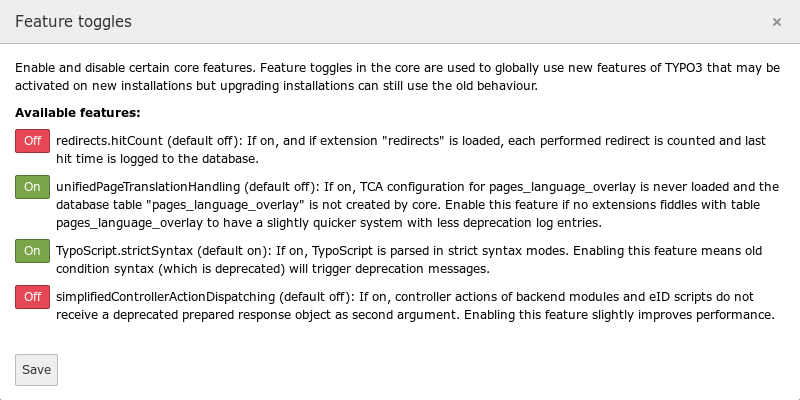
\includegraphics[width=0.70\linewidth]{InDepthChanges/FeatureToggles.png}
	\end{figure}

\end{frame}

% ------------------------------------------------------------------------------
% Feature Toggles

\begin{frame}[fragile]
	\frametitle{Änderungen im System}
	\framesubtitle{Feature Toggles}

	\begin{itemize}
		\item Mit dem Feature Toggle können Entwickler Funktionen parallel zu ihrer
			Vorgängerversion implementieren
		\item Integratoren und Site-Administratoren können entscheiden, wann sie zu den
			neuen Funktionen wechseln möchten
		\item Entwickler können eine API-Klasse einsetzen
		\item Dies bedeutet auch, dass der TYPO3-Kern und die Erweiterungen eine alternative
			Funktionalität für ein bestimmtes Feature bereitstellen können
	\end{itemize}

\end{frame}

% ------------------------------------------------------------------------------
% #85829 - Implement symfony expression language for TypoScript conditions
% #86068 - Deprecate old condition syntax

\begin{frame}[fragile]
	\frametitle{Änderungen im System}
	\framesubtitle{Symfony ExpressionLanguage}

	% decrease font size for code listing
	\lstset{basicstyle=\tiny\ttfamily}

	\begin{itemize}
		\item Die \href{https://symfony.com/doc/current/components/expression_language/syntax.html}{Symfony ExpressionLanguage}
			Komponente wurde für TypoScript-Bedingungen (Frontend
			und Backend) implementiert
		\item Einige Beispiele:

\begin{lstlisting}
[page["uid"] in 18..45]
#  This condition matches, if current page uid is between 18 and 45
[END]

[not ("foo" matches "/bar/")]
# This condition matches, if "foo" does not match the regular expression '/bar/'
[END]

[request.getNormalizedParams().getHttpHost() == 'example.com']
# This condition matches, if current hostname is 'example.com'
[END]
\end{lstlisting}

		\item Die Verwendung der Syntax für alte Bedingungen führt zur Fehlermeldung
	\end{itemize}

\end{frame}

% ------------------------------------------------------------------------------
% #85828 - Move symfony expression language handling into EXT:core

\begin{frame}[fragile]
	\frametitle{Änderungen im System}
	\framesubtitle{Symfony ExpressionLanguage}

	% decrease font size for code listing
	\lstset{basicstyle=\tiny\ttfamily}

	\begin{itemize}
		\item Die ExpressionLanguage kann auch in Ihrem benutzerdefinierten Code verwendet werden
		\item Der TYPO3-Kern enthält die Klasse \texttt{DefaultProvider}, die direkt
			verwendet werden kann (siehe Beispiel unten) und benutzerdefinierte Implementierungen
			können die Klasse \texttt{AbstractProvider} erweitern

\begin{lstlisting}
use \TYPO3\CMS\Core\ExpressionLanguage\DefaultProvider;
use \TYPO3\CMS\Core\ExpressionLanguage\Resolver;

$provider = GeneralUtility::makeInstance(DefaultProvider::class);
$conditionResolver = GeneralUtility::makeInstance(Resolver::class, $provider);
$conditionResolver->evaluate('1 < 2'); // result is true
\end{lstlisting}

	\end{itemize}

\end{frame}

% ------------------------------------------------------------------------------
% #85256 - Install TYPO3 on SQLite

\begin{frame}[fragile]
	\frametitle{Änderungen im System}
	\framesubtitle{TYPO3 auf SQLite installieren}

	\begin{itemize}
		\item TYPO3 unterstützt nun \href{https://www.sqlite.org}{SQLite},
			ein eigenständiges Open-Source SQL-Datenbankmodul
		\item SQLite kann während des webbasierten Installationsprozesses ausgewählt werden,
			wenn das "pdo\_sqlite" installiert und aktiviert ist:
	\end{itemize}

	\begin{figure}
		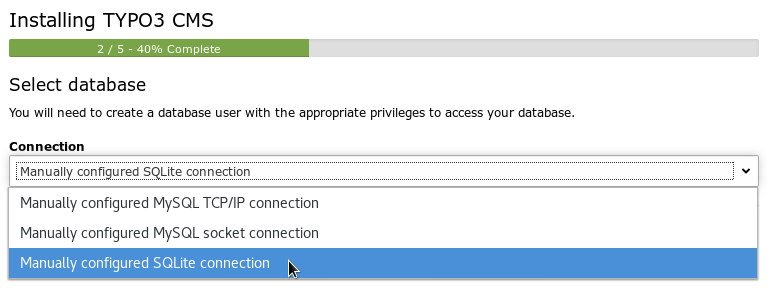
\includegraphics[width=0.65\linewidth]{InDepthChanges/85256-InstallTYPO3OnSQLite.png}
	\end{figure}

\end{frame}
% ------------------------------------------------------------------------------
% #85256 - Install TYPO3 on SQLite

\begin{frame}[fragile]
	\frametitle{Änderungen im System}
	\framesubtitle{TYPO3 auf SQLite installieren}

	\begin{itemize}
		\item Die Datenbank wird in einer einzigen Datei gespeichert, dies bedeutet, dass
			TYPO3-Instanzen jetzt nativ in PHP ausgeführt werden können
		\item Die Verwendung von SQLite ist sinnvoll für relativ kleine TYPO3-Sites
			 oder z. B. für Test- und Entwicklungsinstanzen
		\item Systemadministratoren sollten geeignete Maßnahmen ergreifen, um die Datei
			\texttt{*.sqlite} von unbefügtem Zugriff zu schützen, wenn die Datei im Webcontainer
			gespeichert wird (abhängig vom Installationstyp)
	\end{itemize}

\end{frame}

% ------------------------------------------------------------------------------
% #83461 - Show Fieldname Next To Title In Debug Mode

\begin{frame}[fragile]
	\frametitle{Änderungen im System}
	\framesubtitle{Feldnamen im Debug-Modus}

	\begin{itemize}

		\item TYPO3 Integratoren und Entwickler beschäftigen sich oft mit Eingabefeldern im Backend,
			z.B. bei der Einrichtung von Berechtigungen oder während dem Schreiben von TSConfig.

		\item Anstatt den Quellcode des Browsers zu schauen, werden Feldnamen 
			für jedes Feld angezeigt, das von 
			FormEngine generiert wird

		\item Dies gilt nur für Benutzer mit Administratorrechten und
			erfordert, dass der Debug-Modus in TYPO3 aktiviert wird:

			\smaller
				\texttt{\$GLOBALS['TYPO3\_CONF\_VARS']['BE']['debug']}
			\normalsize

	\end{itemize}

	\begin{figure}
		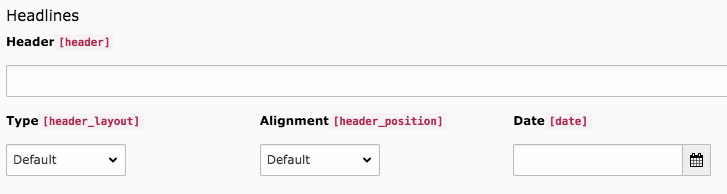
\includegraphics[width=0.60\linewidth]{InDepthChanges/83461-ShowFieldnameNextToTitleInDebugMode.png}
	\end{figure}

\end{frame}

% ------------------------------------------------------------------------------
% Mail Queue (SwiftMailer)

\begin{frame}[fragile]
	\frametitle{Änderungen im System}
	\framesubtitle{Mail Queue}

	% decrease font size for code listing
	\lstset{basicstyle=\tiny\ttfamily}

	\begin{itemize}
		\item Von TYPO3 generierte Emails werden standardmäßig sofort versendet
		\item TYPO3 v9 LTS unterstützt 
			\href{https://example.com}{SwiftMailer's} Funktionalität,
			wo die Nachricht zunächst in einer Warteschlange gespeichert wird und danach verarbeitet wird

		\item Option 1: spool Mails in dem Datenspeicher\newline
			\smaller
				(Emails werden nur dann versendet, wenn die Anfrage ohne Fehler ausgeführt wurde)
			\normalsize

\begin{lstlisting}
$GLOBALS['TYPO3_CONF_VARS']['MAIL']['transport_spool_type'] = 'memory';
\end{lstlisting}

		\item Option 2: spool Mails in Dateien

\begin{lstlisting}
$GLOBALS['TYPO3_CONF_VARS']['MAIL']['transport_spool_type'] = 'file';
$GLOBALS['TYPO3_CONF_VARS']['MAIL']['transport_spool_filepath'] = '/folder/of/choice';
\end{lstlisting}

	\end{itemize}

\end{frame}

% ------------------------------------------------------------------------------
% Mail Queue (SwiftMailer)

\begin{frame}[fragile]
	\frametitle{Änderungen im System}
	\framesubtitle{Mail Queue}

	% decrease font size for code listing
	\lstset{basicstyle=\tiny\ttfamily}

	\begin{itemize}
		\item Der folgende Konsolenbefehl kann verwendet werden, um die Queue zu verarbeiten und
			gespoolte Emails zu senden
			\newline\newline
			\small
				Alle gespoolte Emails verarbeiten:
			\normalsize
\begin{lstlisting}
$ ./typo3/sysext/core/bin/typo3 swiftmailer:spool:send
\end{lstlisting}

			\small
				Nicht mehr als 10 gespoolte Emails verarbeiten:
			\normalsize
\begin{lstlisting}
$ ./typo3/sysext/core/bin/typo3 swiftmailer:spool:send --message-limit=10
\end{lstlisting}

			\small
				Gespoolte Emails verarbeiten, aber nicht länger als 10 Sekunden:
			\normalsize
\begin{lstlisting}
$ ./typo3/sysext/core/bin/typo3 swiftmailer:spool:send --time-limit=10
\end{lstlisting}

	\end{itemize}

\end{frame}

% ------------------------------------------------------------------------------
% Extension Scanner

\begin{frame}[fragile]
	\frametitle{Änderungen im System}
	\framesubtitle{Extension Scanner}

	\begin{itemize}
		\item In TYPO3 wurde ein Extension Scanner hinzugefügt, der helfen soll, TYPO3
			von einer Hauptversion auf die Nächste zu aktualisieren
		\item Dieses Tool kann Erweiterungscode für die Verwendung von TYPO3-Core-APIs prüfen
			die entfernt oder als veraltet markiert wurden
		\item Das Ergebnis ist eine detaillierte Übersicht der erforderlichen Maßnahmen
		\item Falls es zutreffend ist, verweist es auf die entsprechende Dokumentation 
			zur Migration des betreffenden Codes.
		\item Standalone-Tool \href{https://github.com/Tuurlijk/typo3scan}{TYPO3 Scanner}
			(von Michiel Roos)
		\item Weitere Details in einem \href{https://www.youtube.com/watch?v=UdIYDZgBrQU}{Video auf YouTube}
			(von der TYPO3 GmbH)
	\end{itemize}

\end{frame}

% ------------------------------------------------------------------------------
% Extension Scanner

\begin{frame}[fragile]
	\frametitle{Änderungen im System}
	\framesubtitle{Extension Scanner (in TYPO3 v9 LTS)}

	\begin{figure}
		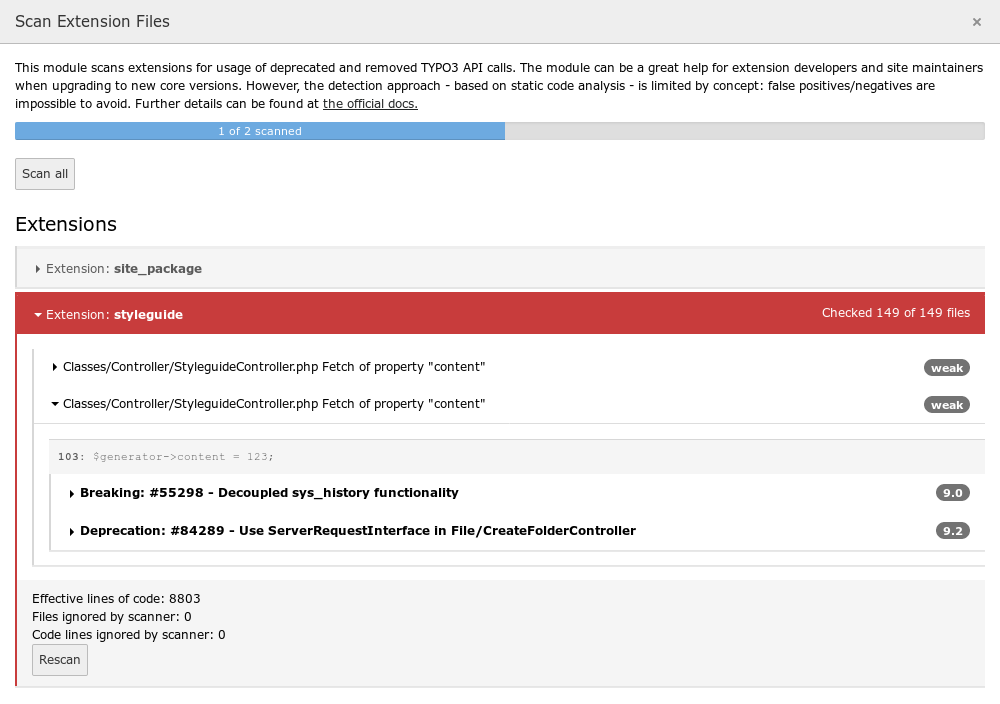
\includegraphics[width=0.70\linewidth]{InDepthChanges/ExtensionScanner.png}
	\end{figure}

\end{frame}

% ------------------------------------------------------------------------------
% Extension Scanner

\begin{frame}[fragile]
	\frametitle{Änderungen im System}
	\framesubtitle{Extension Scanner (Standalone)}

	\begin{figure}
		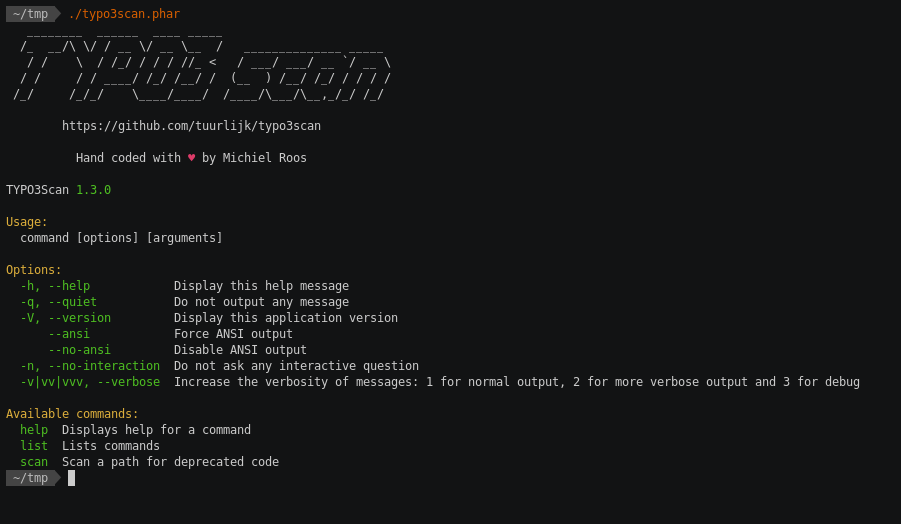
\includegraphics[width=0.70\linewidth]{InDepthChanges/Typo3Scanner.png}
	\end{figure}

\end{frame}

% ------------------------------------------------------------------------------
% #82363 - Make Extbase translation handling consistent with TypoScript

\begin{frame}[fragile]
	\frametitle{In-depth Changes}
	\framesubtitle{Extbase Übersetzung-Handling}

	% decrease font size for code listing
	\lstset{basicstyle=\footnotesize\ttfamily}

	\begin{itemize}
		\item Extbase rendert jetzt übersetzte Datensätze genauso wie 
			TypoScript
		\item Das neue Verhalten wird von einem Schalter gesteuert:

\begin{lstlisting}
config.tx_extbase.features.consistentTranslationOverlayHandling
  = 1
\end{lstlisting}

		\item Das neue Verhalten ist die Standardeinstellung in Version 9 LTS (der Funktionsschalter wird
			in Version 10 entfernt)
		\item Weitere Infos zum Abfragen von Daten mit Extbase in der
			\href{https://github.com/TYPO3/TYPO3.CMS/blob/master/typo3/sysext/core/Documentation/Changelog/9.5/Important-82363-MakeExtBaseTranslationHandlingConsistentWithTyposcript.rst}{TYPO3 Dokumentation}

	\end{itemize}

\end{frame}

% ------------------------------------------------------------------------------
% PSR-3, PSR-7 and PSR-15

\begin{frame}[fragile]
	\frametitle{Änderungen im System}
	\framesubtitle{PHP-Standardempfehlung (PSR)}

	\begin{itemize}
		\item The
			\href{https://www.php-fig.org/psr/}{PHP-Standardempfehlung (PSR)}
			ist eine Spezifikation, die von der PHP Framework Interop Group veröffentlicht wurde
		\item TYPO3 führte PSR-15 Middleware im Frontend und Backend ein
		\item Alle Anfragen rendern im TYPO3-Kern eine Antwort, die mit PSR-7 übereinstimmt 
		\item Der PSR-3-Standard beschreibt eine Protokollierungsschnittstelle für PHP-Anwendungen,
			die von allen Protokollierungsverfahren im gesamten TYPO3-System verwendet
			werden kann
	\end{itemize}

\end{frame}

% ------------------------------------------------------------------------------
